\section[Rail station]{Canberra Station: Dynamic Background and Local Service}
\label{sec:rail}

\subsection{From a fixed reservoir to coupled zones}
Canberra MRT is an elevated, naturally ventilated station in Singapore \cite{canberra-rsp,canberra-lta}. Using its approximate $L=220$ m length with assumed aggregate waiting width $b=6$ m and usable fraction $\alpha=0.8$ gives
\begin{equation}
 A_{\mathrm{occ}}=\alpha Lb=1056\,\mathrm{m^2}.
\label{eq:canberra-area}
\end{equation}
Three access/core/edge zones each have $352\,\mathrm{m^2}$ and, at 4 m effective height, $1408\,\mathrm{m^3}$. Table~\ref{tab:rail-inputs} defines the $33\,^{\circ}\mathrm C$, RH $70\%$ comparison. Its $4$--$10$ h$^{-1}$ background exchange implies 6--15 min replacement times, comparable to the 15-min passenger cycle: storage and humidity feedback must now be resolved.

\begin{figure}[!ht]
\centering
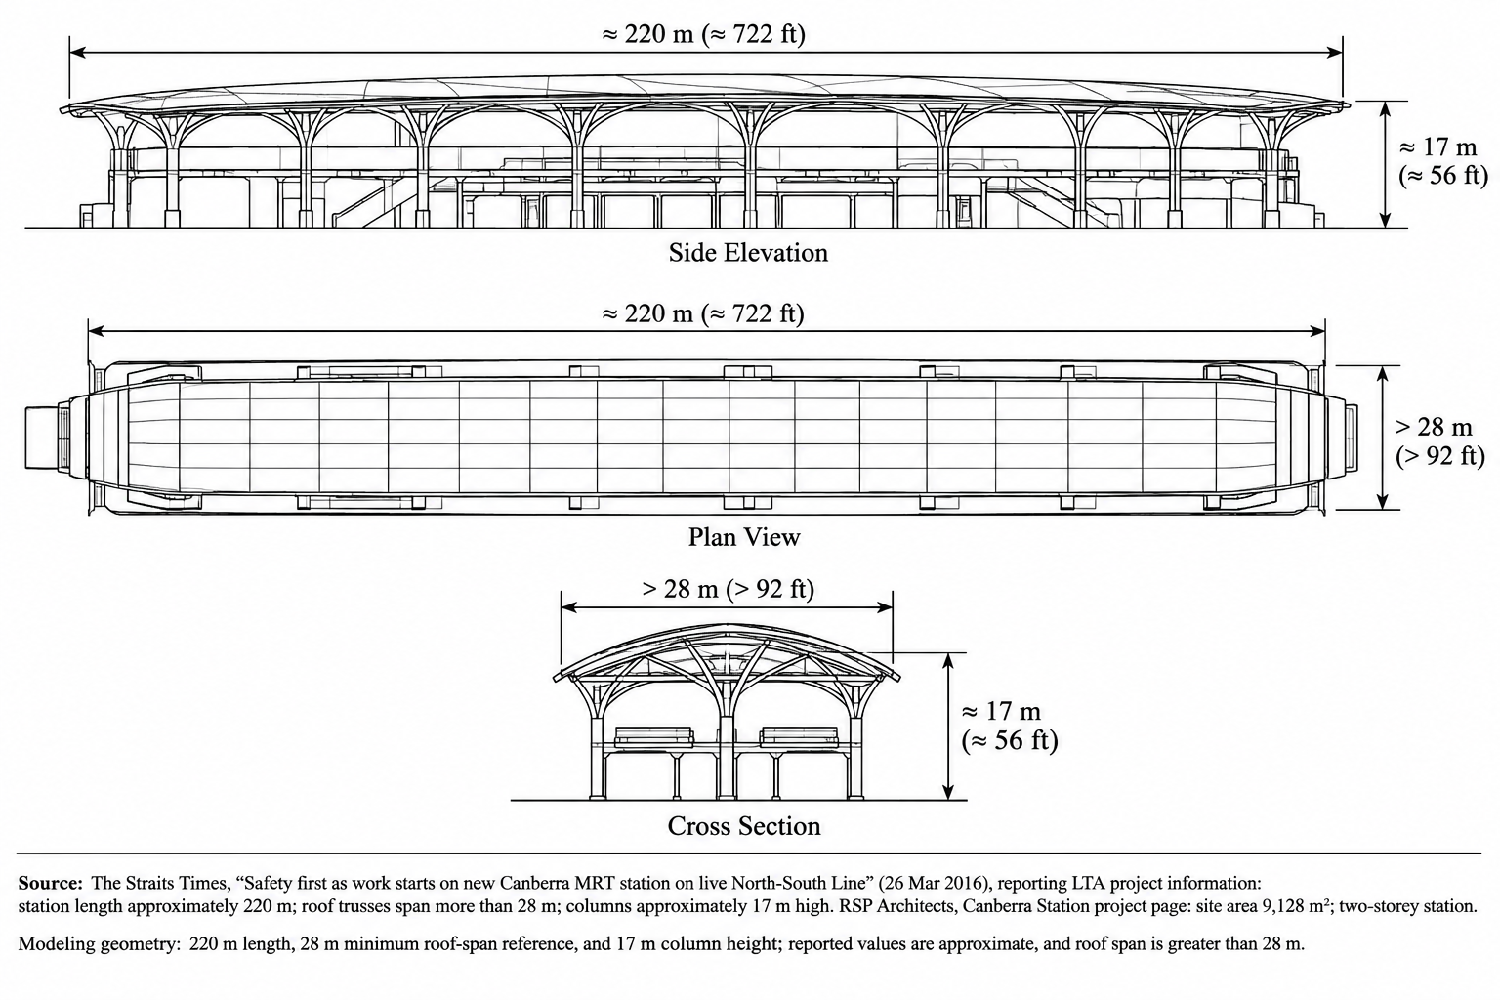
\includegraphics[width=0.66\linewidth]{figures/13_canberra_station.pdf}
\caption{Canberra station context. Structural dimensions guide scale; the three waiting zones are modeled separately \cite{canberra-dimensions,canberra-rsp}.}
\label{fig:canberra}
\end{figure}

Each zone retains $h_z,w_z$ and effective surface temperature $T_{m,z}$, with constant reference dry-air mass $M_z=\rho_{da,o}V_z$. The device, local-mixing and SET operators remain those of the bus. For $x=h$ or $w$, balanced exchange is
\begin{equation}
 \mathcal L_z(x)=\dot m_{0z}(x_o-x_z)+\sum_{j\ne z}\dot m_{zj}(x_j-x_z),
 \qquad \dot m_{0z}=M_z\lambda_z/3600.
\label{eq:rail-exchange}
\end{equation}
$\lambda_z$ is ACH in h$^{-1}$; interzone rates satisfy $\dot m_{zj}=\dot m_{jz}$. Outdoor exchange represents wind/opening effects through the prescribed cycle \cite{ventilation}. With time in seconds, the three conservation equations per zone are \cite{epzone}
\begin{align}
 M_z\dot h_z={}&\mathcal L_z(h)+H_{ma,z}(T_{m,z}-T_z)
 +n_zq_c+n_zg h_v(T_z)+P_z
 +\sum_k x_{zk}\dot m_k(h_{e,zk}-h_z),\label{eq:rail-enthalpy}\\
 M_z\dot w_z={}&\mathcal L_z(w)+n_zg+
 \sum_k x_{zk}\dot m_k(w_{e,zk}-w_z),\label{eq:rail-moisture}\\
 C_{m,z}\dot T_{m,z}={}&H_{mo,z}(T_o-T_{m,z})+Q_{\mathrm{sol},z}
 +n_zq_r-H_{ma,z}(T_{m,z}-T_z).\label{eq:rail-surface}
\end{align}
Here $n_z$ is occupancy; per-person $q_c,q_r$ are convective/radiant W and $g$ is vapor kg/s. Vapor enthalpy is $h_v(T)=2501000+1860T$ J/kg, with no second latent term. $H_{ma},H_{mo}$ are W/K, $C_m$ is J/K, $Q_{\rm sol}$ is W, and $P_z=\sum_kx_{zk}P_k$ with $P_k=1000p_k$ W. Subscript $e$ denotes the unheated device outlet (the bus's $o,s$), so A has no evaporative source; B/C add moisture while approximately conserving outlet enthalpy. Surface exchange cancels between the air and wall budgets.

Recover $T_z=(h_z-2501000w_z)/(1006+1860w_z)$; effective view fraction $F_z$ determines mean radiant temperature \cite{thermalcomfort}:
\begin{equation}
 T_{r,z}=\left[F_z(T_{m,z}+273.15)^4+(1-F_z)(T_{r,o}+273.15)^4\right]^{1/4}-273.15.
\label{eq:rail-mrt}
\end{equation}
The separate outdoor radiant input is $T_{r,o}$. Increasing $w_z$ reduces the next device pass's wet-bulb depression, providing the feedback absent from the fixed-background bus.

\subsection{Local delivery with exact return accounting}
Device flow and entrained background return to their original zone. For finite entrainment ($\beta>0$), the local mixing equations imply
\begin{align}
 (\dot m_k+\dot m_e)(h_{\ell,zk}-h_z)+(1-\chi)P_k
 &=\dot m_k(h_{e,zk}-h_z)+P_k,\\
 (\dot m_k+\dot m_e)(w_{\ell,zk}-w_z)
 &=\dot m_k(w_{e,zk}-w_z).
\label{eq:return-closure}
\end{align}
Thus the local exposure calculation preserves the existing net heat and moisture sources exactly. Covered people use local $T,\phi,v$; uncovered people use background $T,\phi,v_0$, and both share $T_r$. Here $\beta=0.5$, $\chi=1$ and A/B/C unit flows are $0.6/0.6/1.2$ kg dry air/s under Table~\ref{tab:rail-inputs}; $\chi=1$ places all electrical heat in supply before passengers.

Two reductions identify the inheritance precisely. At $\beta=0$, the scalar exposure becomes the original shared-background calculation while prescribed speeds remain. Fixing background to outdoor $h_a,w_a$, using bus radiation, speeds, occupancy and $\beta$, and setting $\chi=0$ recovers the bus calculation exactly. Setting time derivatives to zero alone would not impose that reservoir boundary.

\subsection{Counts, coverage and efficiency}
Let $s$ index an installation and $x_{zk}$ its nonnegative integer count of type $k$ in zone $z$. For unit footprints $a_{A/B/C}=20/30/40\,\mathrm{m^2}$, uniform zone density gives
\begin{equation}
 c_{zk}=\frac{x_{zk}a_k}{A_z},\qquad
 c_{z0}=1-\sum_k c_{zk}\ge0,\qquad \sum_kx_{zk}a_k\le A_z.
\label{eq:coverage}
\end{equation}
These passenger fractions $c$ differ from the air-mixing fraction $\beta$. Average discomfort across subgroups, not velocities or device efficiencies:
\begin{equation}
 \overline D_{s,z}(t)=c_{z0}D[\Theta(T_z,T_{r,z},v_0,\phi_z)]
 +\sum_k c_{zk}D[\Theta(T_{\ell,zk},T_{r,z},v_{zk},\phi_{\ell,zk})].
\label{eq:mixed-discomfort}
\end{equation}
All units affect the background; direct coverage determines the additional local exposure. Every plan starts after the same two-hour uncooled warm-up, runs two hours, and uses a matched no-device baseline. The common passenger history totals 440 person-hours. With $p_k$ in kW,
\begin{align}
 U_s&=\frac1{3600}\int_0^{7200}\sum_z n_z(t)[D_{0,z}(t)-\overline D_{s,z}(t)]\,dt,\\
 E_s&=\frac1{3600}\int_0^{7200}\sum_{z,k}x_{zk}p_k\,dt,
 \qquad \eta_s=U_s/E_s.
\label{eq:rail-efficiency}
\end{align}
The $1/3600$ factors convert seconds to hours, retaining person$\cdot{}^{\circ}\mathrm C\cdot$h/kWh. This section compares $U/E$. Mean residual $\overline R_s=\int\sum_z n_z\overline D_{s,z}\,dt/\int\sum_z n_z\,dt$ supplies the later adequacy criterion in Section~\ref{sec:effectiveness}.

\subsection{Deployment results and verification}
Among 24 sampled plans, A3 maximizes $\eta$ at $37.58$; among the six equal-$68.18\%$-coverage benchmarks, A36 leads at $35.49$. The distinct candidate sets answer scale and device-comparison questions, respectively (Figure~\ref{fig:deployment-efficiency}).

Plan suffixes give total device counts. For A36/B24/C18/AB30/AC27/ABC24, per-zone $(A,B,C)$ counts are $(12,0,0)$, $(0,8,0)$, $(0,0,6)$, $(6,4,0)$, $(6,0,3)$ and $(3,2,3)$, respectively; A3 places one fan in each zone.

\begin{table}[!ht]
\centering\small
\caption{Nominal efficiency accounting: $U$ in person$\cdot{}^{\circ}$C$\cdot$h, $E$ in kWh.}
\label{tab:deployment-results}
\begin{tabular}{@{}lrrrr@{}}
\toprule
Plan & Person-time coverage & $U$ & $E$ & $\eta$\\
\midrule
A3 & 5.68\% & 56.38 & 1.5 & 37.58\\
A36 & 68.18\% & 638.89 & 18.0 & 35.49\\
B24 & 68.18\% & 446.28 & 57.6 & 7.75\\
C18 & 68.18\% & 453.00 & 90.0 & 5.03\\
AB30 & 68.18\% & 581.61 & 37.8 & 15.39\\
AC27 & 68.18\% & 593.68 & 54.0 & 10.99\\
ABC24 & 68.18\% & 524.76 & 63.9 & 8.21\\
AB30-R & 76.19\% & 695.07 & 37.8 & 18.39\\
\bottomrule
\end{tabular}
\end{table}

Redistributing AB30's 18 A and 12 B units to zone counts $(3,4,0)$, $(12,3,0)$ and $(3,5,0)$ raises person-time coverage from $68.18\%$ to $76.19\%$. At the same 37.8 kWh, $U$ rises from $581.61$ to $695.07$ and $\eta$ from $15.39$ to $18.39$: allocation changes useful delivery without adding equipment.

A36 retains its equal-coverage efficiency lead for all 15 combinations $\beta=0/0.25/0.5/0.75/1$, $\chi=0/0.5/1$. Varying A's unit flow through $0.3/0.6/1.2$ kg dry air/s gives efficiencies $34.06/35.49/36.22$. Figure~\ref{fig:local-sensitivity} shows the controlled delivery sensitivity.


\begin{figure}[!ht]
\centering
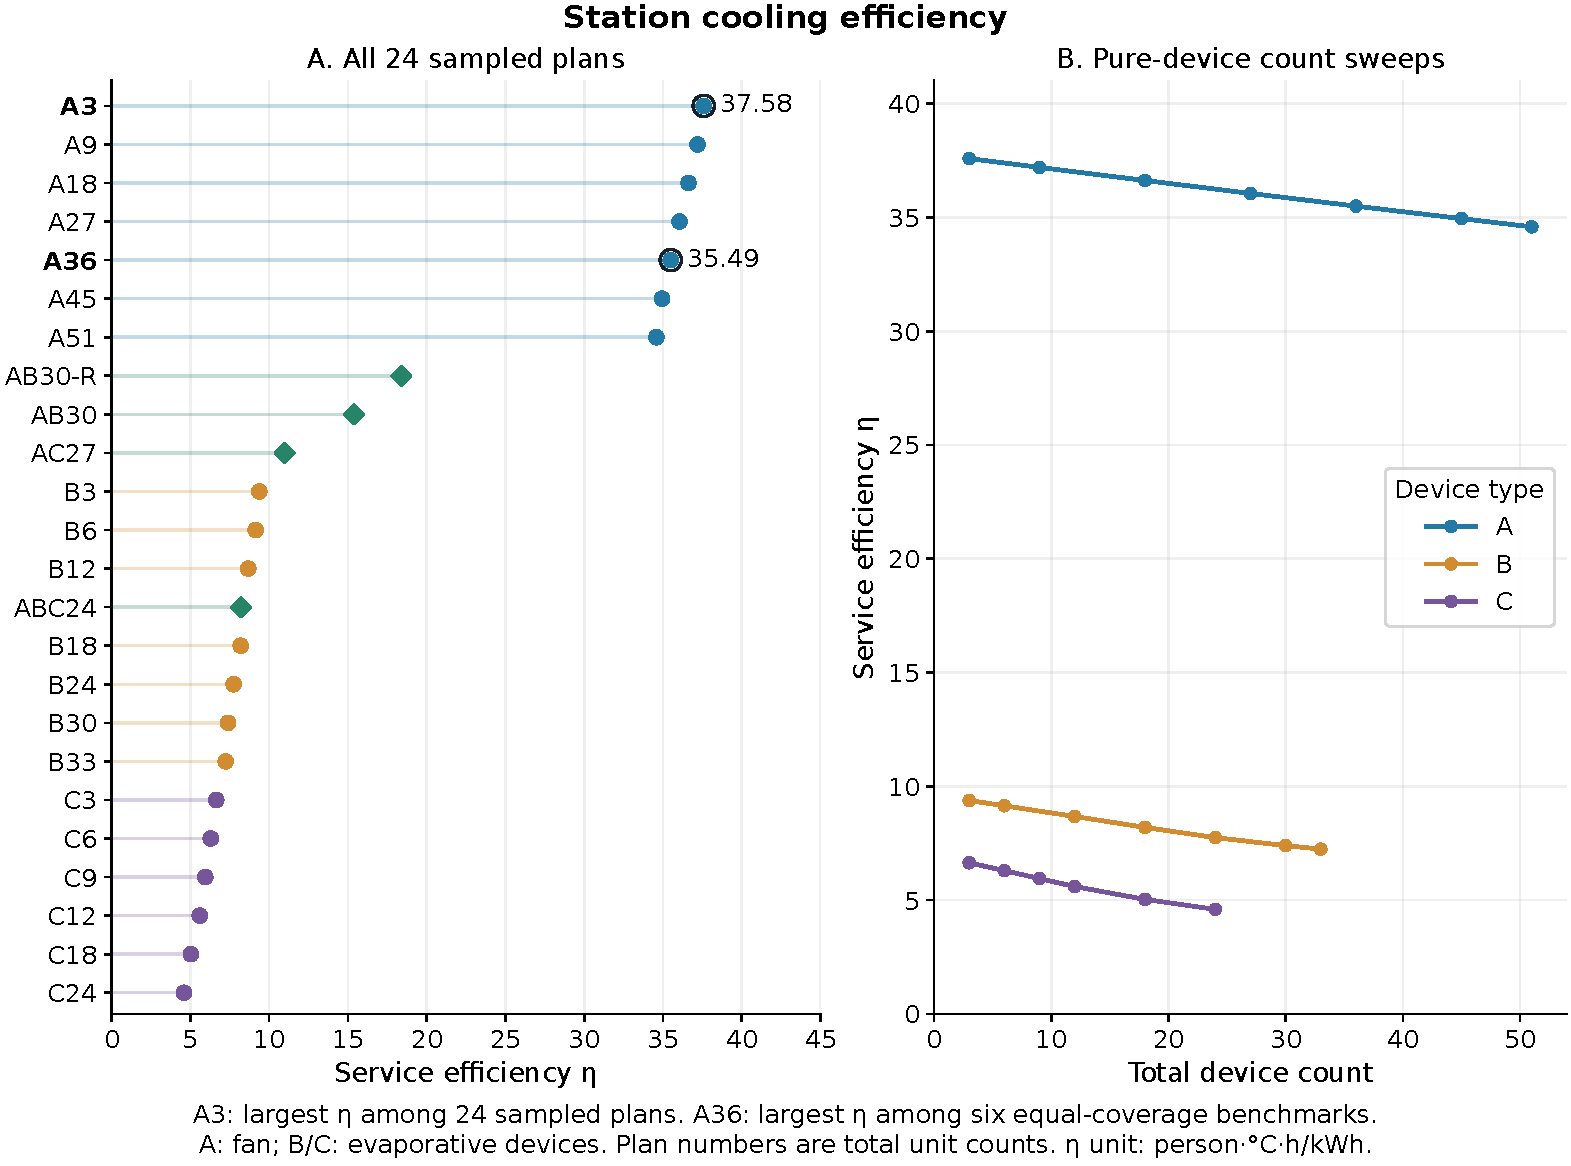
\includegraphics[width=0.88\linewidth]{figures/22_station_efficiency.pdf}
\caption{A3 leads all 24 sampled installations; A36 leads the six equal-coverage benchmarks. Device counts change both delivered service and background loads.}
\label{fig:deployment-efficiency}
\end{figure}

\begin{figure}[!ht]
\centering
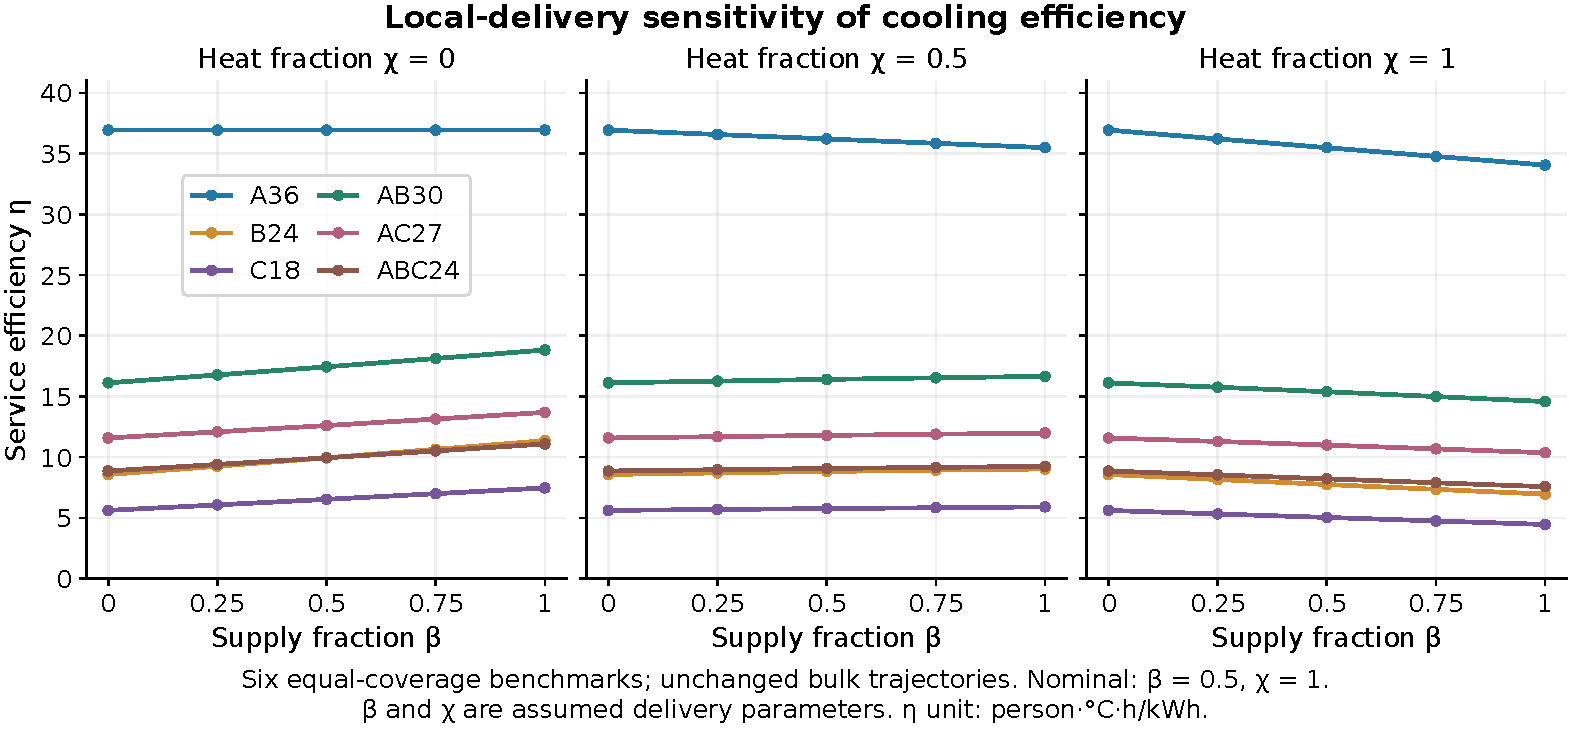
\includegraphics[width=0.88\linewidth]{figures/23_delivery_efficiency.pdf}
\caption{Efficiency sensitivity to mixing and heat allocation; background trajectories remain unchanged by the local mapping.}
\label{fig:local-sensitivity}
\end{figure}

Global energy/moisture budgets and local return identities close numerically. Halving the time step changes the tested mixed-plan efficiencies by at most $5.4\times10^{-6}$ relatively; $\beta=0$ reproduces all 24 former shared-background results exactly. The fixed-reservoir test recovers bus states and service. These checks verify the extension's conservation and reduction properties.
